\subsection{Landmines}

The selection of sensing hardware in our multi-drone landmine detection system relies on a clear understanding of the target: landmines. Landmines differ widely in size, materials, triggering mechanisms, and intended targets. These physical differences strongly affect how detectable they are, especially when using drones with limited payload capacity. This section outlines the main landmine types and highlights the features that influence detection. This overview supports informed decisions on sensor selection and data acquisition in our system.

Landmines are commonly classified into two main categories based on their intended targets: anti-tank landmines (ATLs) and anti-personnel landmines (APLs).
\footnote{\url{https://en.wikipedia.org/wiki/Land_mine}}

ATLs are designed to disable or destroy heavy vehicles such as tanks or armored transports. They are typically large, with diameters ranging from 13 to 40 cm, and contain 6 to 11 kg of explosives\cite{paik2002image}. These mines are generally triggered by high pressures and are often buried beneath roadways or terrain. Traditional ATLs use metal casings, but modern designs may incorporate plastic or composite materials to reduce detectability \cite{evans2024detection}. Based on their activation mechanisms, ATLs can be classified into pressure-activated blast mines, tilt-rod or magnetic mines, and side-attack mines.

APLs are intended to injure or kill individuals on foot. They are much smaller than ATLs, typically ranging from 6 to 15 cm in diameter, and contain only 0.1 to 4 kg of explosives\cite{paik2002image}. These mines are triggered by very low pressure, often below 10 kg, which makes them highly dangerous and difficult to detect. APLs are commonly constructed from plastic, rubber, or other low-metal-content materials, further reducing their detectability \cite{kaya2017buried}. Like ATLs, APLs are also divided into subtypes, including blasting mines, bounding fragmentation mines, and directional fragmentation mines.

\begin{figure}[h]
    \centering
    \begin{subfigure}[b]{0.24\textwidth}
        \centering
        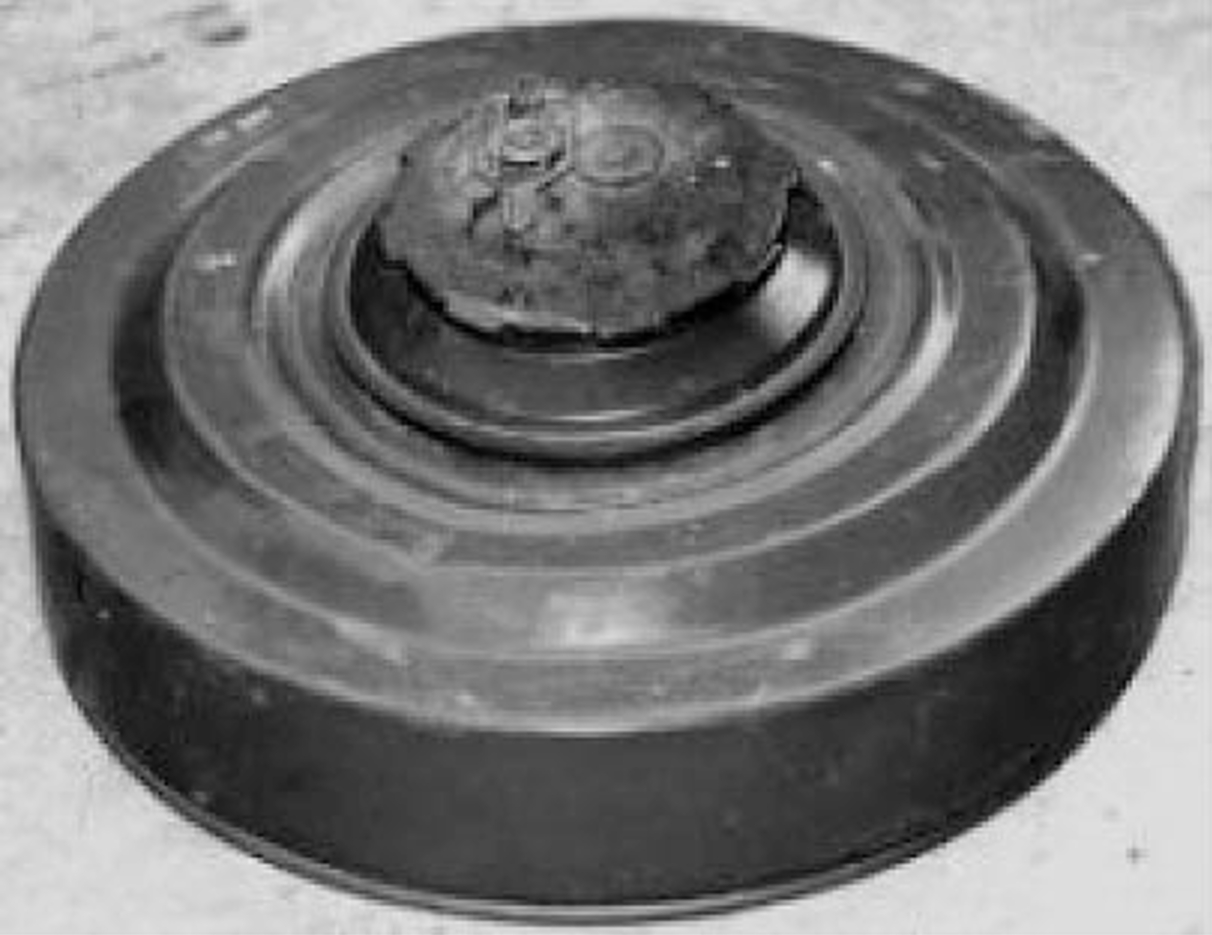
\includegraphics[height=2cm]{figs/Huirui/tm62m.png}
        \subcaption*{(a)}
    \end{subfigure}
    \begin{subfigure}[b]{0.24\textwidth}
        \centering
        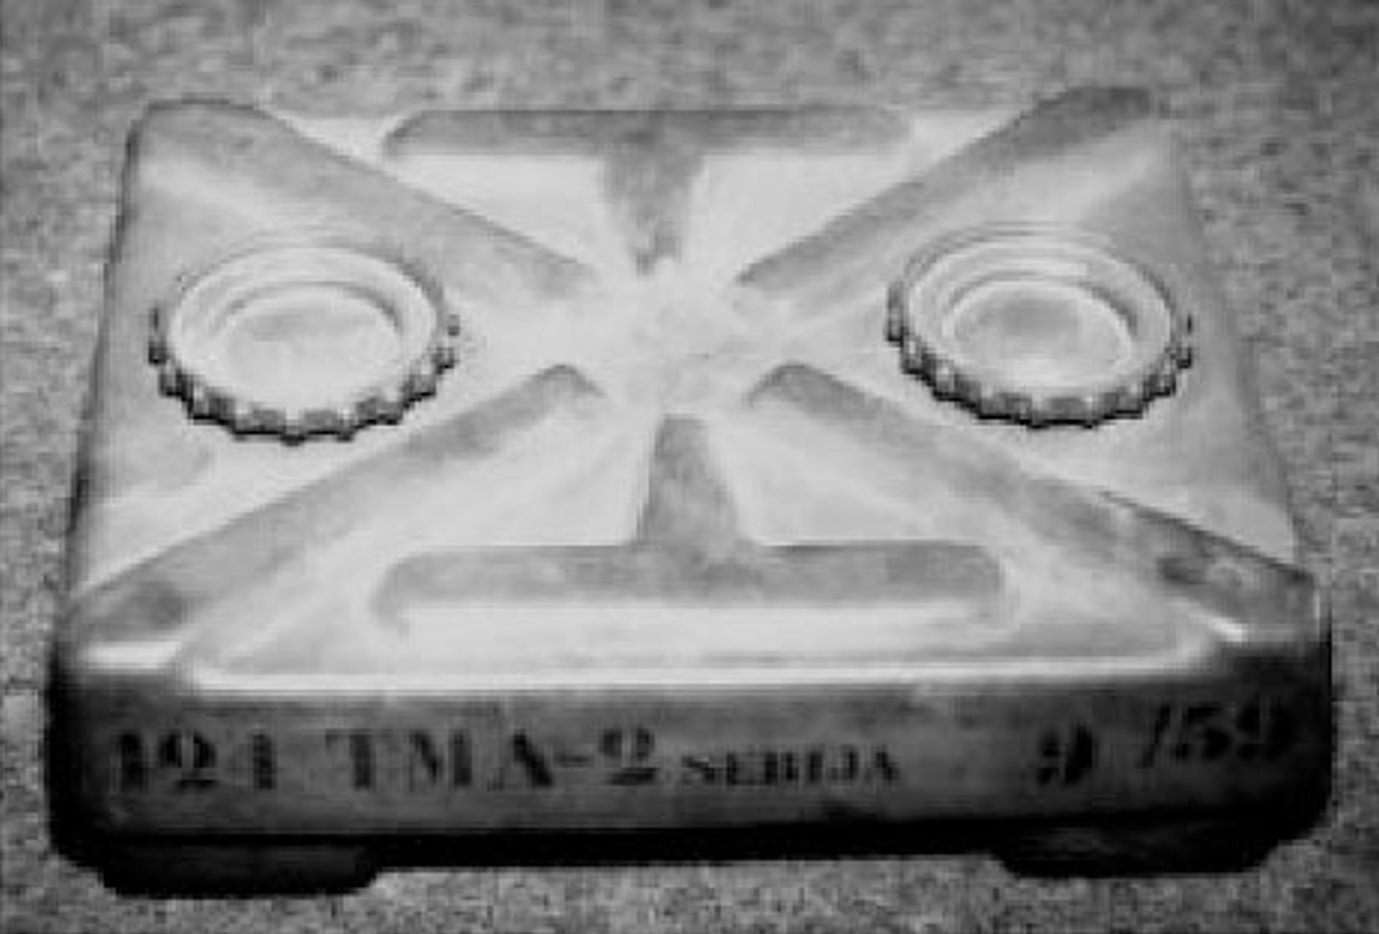
\includegraphics[height=2cm]{figs/Huirui/tma2.png}
        \subcaption*{(b)}
    \end{subfigure}
    \begin{subfigure}[b]{0.24\textwidth}
        \centering
        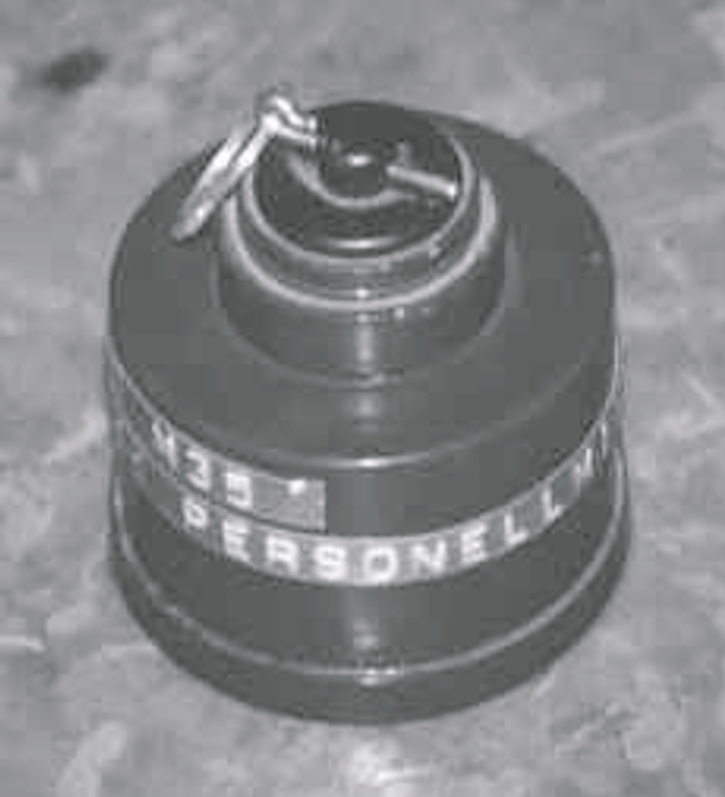
\includegraphics[height=2cm]{figs/Huirui/prbm35.png}
        \subcaption*{(c)}
    \end{subfigure}
    \begin{subfigure}[b]{0.24\textwidth}
        \centering
        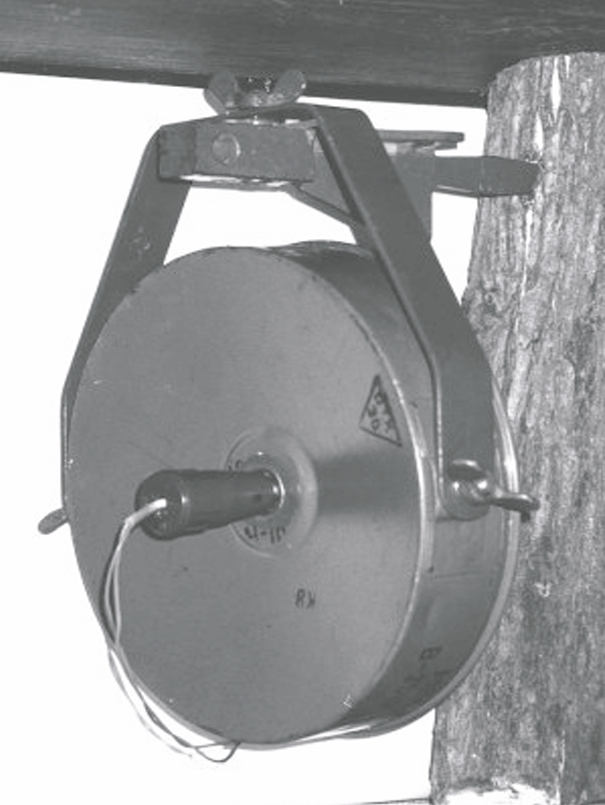
\includegraphics[height=2cm]{figs/Huirui/mon100.png}
        \subcaption*{(d)}
    \end{subfigure}

    \caption{Typical ATLs and APLs: (a) TM-62M, (b) TMA-2, (c) PRB-M35, and (d) MON-100~\cite{paik2002image}.}
    \label{fig:mine_examples}
\end{figure}


\begin{table}[h]
    \centering
    \small
    \renewcommand{\arraystretch}{1.3}
    \caption{Specifications for selected ATLs and APLs~\cite{paik2002image}.}
    \label{tab:mine_specs}
    \begin{tabular}{l p{2.8cm} p{2.8cm} p{2.8cm} p{2.8cm}}
        \toprule
        \textbf{Model No.} & \textbf{TM-62M} & \textbf{TMA-2} & \textbf{PRB-M35} & \textbf{MON-100} \\
        \midrule
        Type & ATL & ATL & APL & APL \\
        Height (cm) & 11.2 & 14.0 & 5.7 & 8.2 \\
        Diameter / Width (cm) & 31.6 & 26.0 × 20.0 & 6.4 & 23.6 \\
        Weight (kg) & 8.5 & 7.5 & 0.16 & 5.0 \\
        Material & Steel & Plastic & Plastic & Steel \\
        Sensitivity & 200 kg & 120 kg & 8 kg & Depends on fuses \\
        \bottomrule
    \end{tabular}
\end{table}

Figure~\ref{fig:mine_examples} shows four representative examples of ATLs and APLs, and Table~\ref{tab:mine_specs} summarizes their key structural specifications. As the table indicates, both ATLs and APLs can be constructed from metallic, low-metallic, or non-metallic materials. However, APLs are significantly smaller in size, which make them more difficult to detect, especially from aerial platforms. And from a technical perspective, a system capable of reliably detecting small APLs is also likely to detect the larger ATLs. Also, nowadays APLs are more responsible for the vast majority of civilian injuries and deaths in post-conflict areas compared with ATLs \cite{unmas2021handbook}, which underscores their humanitarian significance. For these reasons, our project focuses on the detection of anti-personnel landmines.
